\documentclass{standalone}
\usepackage{tikz}
\usetikzlibrary{patterns, positioning}


\begin{document}
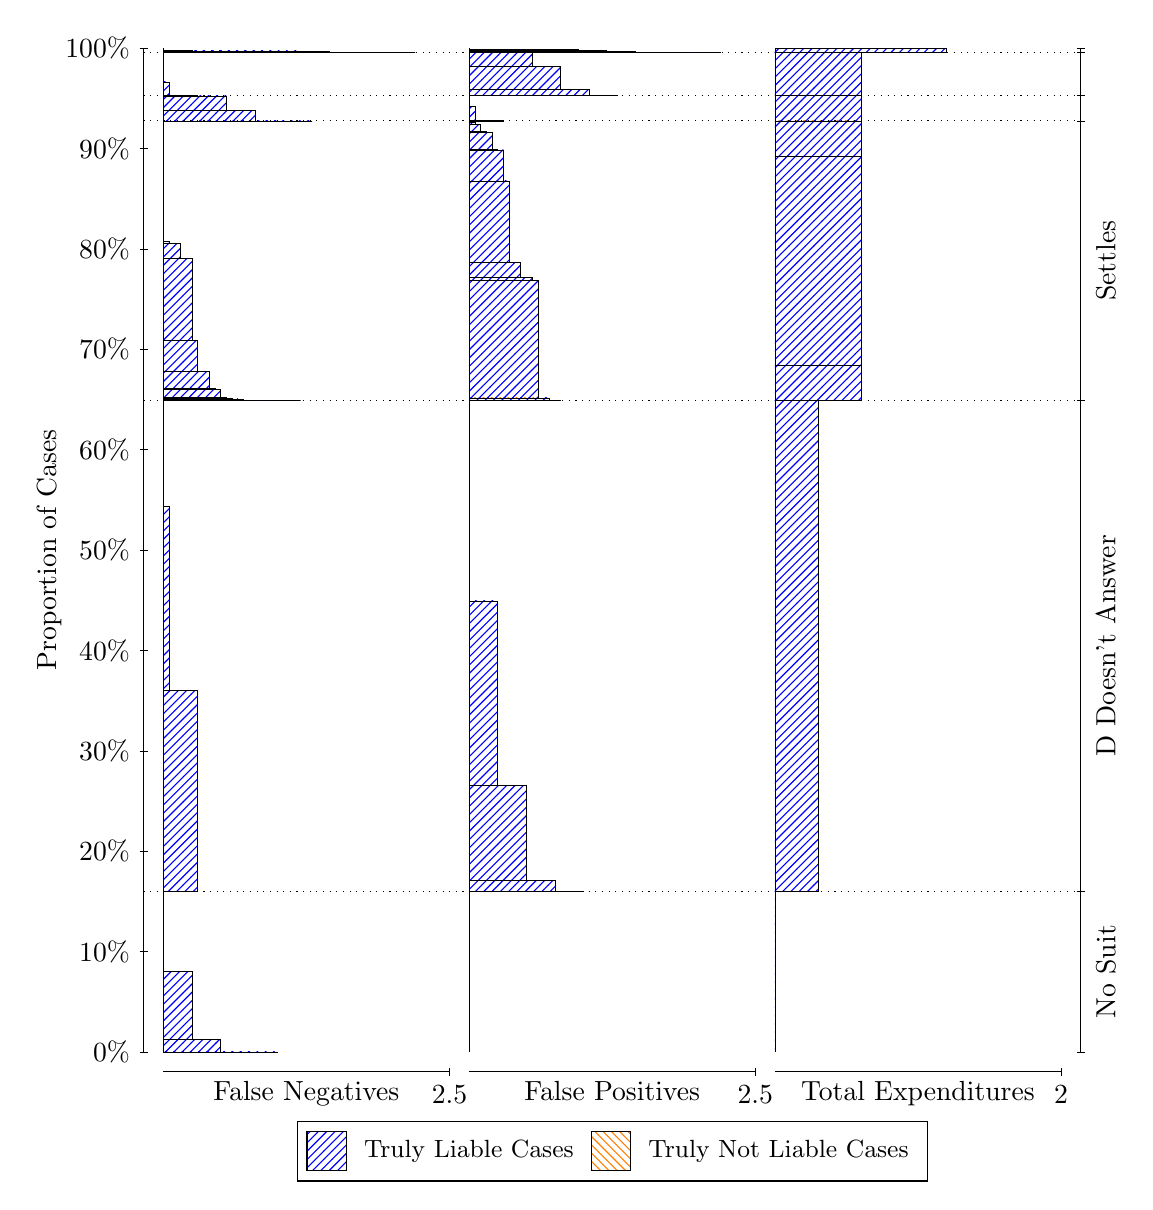
\begin{tikzpicture}
\draw[black, very thin] (1.5,1.75) -- (1.5,14.5);
\node[rotate=90, text=black, anchor=center] at (0.3, 8.125) {Proportion of Cases};
\draw[black, very thin] (1.45,1.75) -- (1.55,1.75);
\node[text=black, anchor=east] at (1.45, 1.75) {0\%};
\draw[black, very thin] (1.45,3.025) -- (1.55,3.025);
\node[text=black, anchor=east] at (1.45, 3.025) {10\%};
\draw[black, very thin] (1.45,4.3) -- (1.55,4.3);
\node[text=black, anchor=east] at (1.45, 4.3) {20\%};
\draw[black, very thin] (1.45,5.575) -- (1.55,5.575);
\node[text=black, anchor=east] at (1.45, 5.575) {30\%};
\draw[black, very thin] (1.45,6.85) -- (1.55,6.85);
\node[text=black, anchor=east] at (1.45, 6.85) {40\%};
\draw[black, very thin] (1.45,8.125) -- (1.55,8.125);
\node[text=black, anchor=east] at (1.45, 8.125) {50\%};
\draw[black, very thin] (1.45,9.4) -- (1.55,9.4);
\node[text=black, anchor=east] at (1.45, 9.4) {60\%};
\draw[black, very thin] (1.45,10.675) -- (1.55,10.675);
\node[text=black, anchor=east] at (1.45, 10.675) {70\%};
\draw[black, very thin] (1.45,11.95) -- (1.55,11.95);
\node[text=black, anchor=east] at (1.45, 11.95) {80\%};
\draw[black, very thin] (1.45,13.225) -- (1.55,13.225);
\node[text=black, anchor=east] at (1.45, 13.225) {90\%};
\draw[black, very thin] (1.45,14.5) -- (1.55,14.5);
\node[text=black, anchor=east] at (1.45, 14.5) {100\%};

\draw[black, very thin] (13.4,1.75) -- (13.4,14.5);
\draw[black, very thin] (13.35,1.75) -- (13.45,1.75);
\node[anchor=west] at (13.35, 1.75) {};
\draw[black, very thin] (13.35,3.7895) -- (13.45,3.7895);
\node[anchor=west] at (13.35, 3.7895) {};
\draw[black, very thin] (13.35,10.027) -- (13.45,10.027);
\node[anchor=west] at (13.35, 10.027) {};
\draw[black, very thin] (13.35,13.574) -- (13.45,13.574);
\node[anchor=west] at (13.35, 13.574) {};
\draw[black, very thin] (13.35,13.894) -- (13.45,13.894);
\node[anchor=west] at (13.35, 13.894) {};
\draw[black, very thin] (13.35,14.444) -- (13.45,14.444);
\node[anchor=west] at (13.35, 14.444) {};
\draw[black, very thin] (13.35,14.5) -- (13.45,14.5);
\node[anchor=west] at (13.35, 14.5) {};

\draw[black, very thin, pattern color=blue, pattern=north east lines] (1.75,1.75) rectangle (3.2033,1.75);
\draw[black, very thin, pattern color=blue, pattern=north east lines] (1.75,1.75) rectangle (2.84,1.7514);
\draw[black, very thin, pattern color=blue, pattern=north east lines] (1.75,1.7514) rectangle (2.4767,1.9132);
\draw[black, very thin, pattern color=blue, pattern=north east lines] (1.75,1.9132) rectangle (2.1133,2.7712);
\draw[black, very thin, pattern color=orange, pattern=north west lines] (1.75,2.7712) rectangle (1.75,2.7712);
\draw[black, very thin, pattern color=blue, pattern=north east lines] (1.75,2.7712) rectangle (1.75,3.7895);
\draw[black, very thin, pattern color=blue, pattern=north east lines] (1.75,3.7895) rectangle (2.186,6.3374);
\draw[black, very thin, pattern color=blue, pattern=north east lines] (1.75,6.3374) rectangle (1.8227,8.682);
\draw[black, very thin, pattern color=orange, pattern=north west lines] (1.75,8.682) rectangle (1.75,8.682);
\draw[black, very thin, pattern color=blue, pattern=north east lines] (1.75,8.682) rectangle (1.75,10.027);
\draw[black, very thin, pattern color=blue, pattern=north east lines] (1.75,10.027) rectangle (3.494,10.027);
\draw[black, very thin, pattern color=blue, pattern=north east lines] (1.75,10.027) rectangle (3.3487,10.027);
\draw[black, very thin, pattern color=blue, pattern=north east lines] (1.75,10.027) rectangle (3.2033,10.027);
\draw[black, very thin, pattern color=blue, pattern=north east lines] (1.75,10.027) rectangle (3.1307,10.027);
\draw[black, very thin, pattern color=blue, pattern=north east lines] (1.75,10.027) rectangle (3.058,10.027);
\draw[black, very thin, pattern color=blue, pattern=north east lines] (1.75,10.027) rectangle (2.9853,10.027);
\draw[black, very thin, pattern color=blue, pattern=north east lines] (1.75,10.027) rectangle (2.9127,10.027);
\draw[black, very thin, pattern color=blue, pattern=north east lines] (1.75,10.027) rectangle (2.84,10.028);
\draw[black, very thin, pattern color=blue, pattern=north east lines] (1.75,10.028) rectangle (2.7673,10.037);
\draw[black, very thin, pattern color=blue, pattern=north east lines] (1.75,10.037) rectangle (2.6947,10.044);
\draw[black, very thin, pattern color=blue, pattern=north east lines] (1.75,10.044) rectangle (2.622,10.047);
\draw[black, very thin, pattern color=blue, pattern=north east lines] (1.75,10.047) rectangle (2.5493,10.067);
\draw[black, very thin, pattern color=blue, pattern=north east lines] (1.75,10.067) rectangle (2.4767,10.162);
\draw[black, very thin, pattern color=blue, pattern=north east lines] (1.75,10.162) rectangle (2.404,10.173);
\draw[black, very thin, pattern color=blue, pattern=north east lines] (1.75,10.173) rectangle (2.3313,10.391);
\draw[black, very thin, pattern color=blue, pattern=north east lines] (1.75,10.391) rectangle (2.2587,10.393);
\draw[black, very thin, pattern color=blue, pattern=north east lines] (1.75,10.393) rectangle (2.186,10.787);
\draw[black, very thin, pattern color=blue, pattern=north east lines] (1.75,10.787) rectangle (2.1133,11.824);
\draw[black, very thin, pattern color=blue, pattern=north east lines] (1.75,11.824) rectangle (2.0407,11.824);
\draw[black, very thin, pattern color=blue, pattern=north east lines] (1.75,11.824) rectangle (1.968,12.016);
\draw[black, very thin, pattern color=blue, pattern=north east lines] (1.75,12.016) rectangle (1.8953,12.016);
\draw[black, very thin, pattern color=blue, pattern=north east lines] (1.75,12.016) rectangle (1.8227,12.047);
\draw[black, very thin, pattern color=orange, pattern=north west lines] (1.75,12.047) rectangle (1.75,12.047);
\draw[black, very thin, pattern color=blue, pattern=north east lines] (1.75,12.047) rectangle (1.75,13.574);
\draw[black, very thin, pattern color=blue, pattern=north east lines] (1.75,13.574) rectangle (3.6393,13.574);
\draw[black, very thin, pattern color=blue, pattern=north east lines] (1.75,13.574) rectangle (3.276,13.574);
\draw[black, very thin, pattern color=blue, pattern=north east lines] (1.75,13.574) rectangle (2.9127,13.711);
\draw[black, very thin, pattern color=blue, pattern=north east lines] (1.75,13.711) rectangle (2.5493,13.891);
\draw[black, very thin, pattern color=blue, pattern=north east lines] (1.75,13.891) rectangle (2.186,13.894);
\draw[black, very thin, pattern color=orange, pattern=north west lines] (1.75,13.894) rectangle (1.75,13.894);
\draw[black, very thin, pattern color=blue, pattern=north east lines] (1.75,13.894) rectangle (2.186,13.896);
\draw[black, very thin, pattern color=blue, pattern=north east lines] (1.75,13.896) rectangle (1.8227,14.069);
\draw[black, very thin, pattern color=orange, pattern=north west lines] (1.75,14.069) rectangle (1.75,14.069);
\draw[black, very thin, pattern color=blue, pattern=north east lines] (1.75,14.069) rectangle (1.75,14.444);
\draw[black, very thin, pattern color=blue, pattern=north east lines] (1.75,14.444) rectangle (4.9473,14.444);
\draw[black, very thin, pattern color=blue, pattern=north east lines] (1.75,14.444) rectangle (4.584,14.444);
\draw[black, very thin, pattern color=blue, pattern=north east lines] (1.75,14.444) rectangle (4.2207,14.445);
\draw[black, very thin, pattern color=blue, pattern=north east lines] (1.75,14.445) rectangle (3.8573,14.453);
\draw[black, very thin, pattern color=blue, pattern=north east lines] (1.75,14.453) rectangle (3.494,14.464);
\draw[black, very thin, pattern color=blue, pattern=north east lines] (1.75,14.464) rectangle (3.1307,14.465);
\draw[black, very thin, pattern color=blue, pattern=north east lines] (1.75,14.465) rectangle (2.84,14.465);
\draw[black, very thin, pattern color=blue, pattern=north east lines] (1.75,14.465) rectangle (2.7673,14.465);
\draw[black, very thin, pattern color=blue, pattern=north east lines] (1.75,14.465) rectangle (2.4767,14.465);
\draw[black, very thin, pattern color=blue, pattern=north east lines] (1.75,14.465) rectangle (2.1133,14.47);
\draw[black, very thin, pattern color=orange, pattern=north west lines] (1.75,14.47) rectangle (1.75,14.47);
\draw[black, very thin, pattern color=blue, pattern=north east lines] (1.75,14.47) rectangle (1.75,14.5);
\draw[black, very thin, pattern color=orange, pattern=north west lines] (5.6333,1.75) rectangle (5.6333,1.75);
\draw[black, very thin, pattern color=blue, pattern=north east lines] (5.6333,1.75) rectangle (5.6333,3.7895);
\draw[black, very thin, pattern color=orange, pattern=north west lines] (5.6333,3.7895) rectangle (7.0867,3.7895);
\draw[black, very thin, pattern color=blue, pattern=north east lines] (5.6333,3.7895) rectangle (7.0867,3.7909);
\draw[black, very thin, pattern color=blue, pattern=north east lines] (5.6333,3.7909) rectangle (6.7233,3.9337);
\draw[black, very thin, pattern color=blue, pattern=north east lines] (5.6333,3.9337) rectangle (6.36,5.1342);
\draw[black, very thin, pattern color=blue, pattern=north east lines] (5.6333,5.1342) rectangle (5.9967,7.4788);
\draw[black, very thin, pattern color=blue, pattern=north east lines] (5.6333,7.4788) rectangle (5.6333,10.027);
\draw[black, very thin, pattern color=orange, pattern=north west lines] (5.6333,10.027) rectangle (6.796,10.027);
\draw[black, very thin, pattern color=blue, pattern=north east lines] (5.6333,10.027) rectangle (6.796,10.027);
\draw[black, very thin, pattern color=orange, pattern=north west lines] (5.6333,10.027) rectangle (6.6507,10.027);
\draw[black, very thin, pattern color=blue, pattern=north east lines] (5.6333,10.027) rectangle (6.6507,10.056);
\draw[black, very thin, pattern color=orange, pattern=north west lines] (5.6333,10.056) rectangle (6.5053,10.056);
\draw[black, very thin, pattern color=blue, pattern=north east lines] (5.6333,10.056) rectangle (6.5053,11.553);
\draw[black, very thin, pattern color=blue, pattern=north east lines] (5.6333,11.553) rectangle (6.4327,11.585);
\draw[black, very thin, pattern color=orange, pattern=north west lines] (5.6333,11.585) rectangle (6.36,11.585);
\draw[black, very thin, pattern color=blue, pattern=north east lines] (5.6333,11.585) rectangle (6.36,11.585);
\draw[black, very thin, pattern color=blue, pattern=north east lines] (5.6333,11.585) rectangle (6.2873,11.776);
\draw[black, very thin, pattern color=orange, pattern=north west lines] (5.6333,11.776) rectangle (6.2147,11.776);
\draw[black, very thin, pattern color=blue, pattern=north east lines] (5.6333,11.776) rectangle (6.2147,11.777);
\draw[black, very thin, pattern color=blue, pattern=north east lines] (5.6333,11.777) rectangle (6.142,12.813);
\draw[black, very thin, pattern color=blue, pattern=north east lines] (5.6333,12.813) rectangle (6.0693,13.207);
\draw[black, very thin, pattern color=blue, pattern=north east lines] (5.6333,13.207) rectangle (5.9967,13.21);
\draw[black, very thin, pattern color=blue, pattern=north east lines] (5.6333,13.21) rectangle (5.924,13.427);
\draw[black, very thin, pattern color=blue, pattern=north east lines] (5.6333,13.427) rectangle (5.8513,13.438);
\draw[black, very thin, pattern color=blue, pattern=north east lines] (5.6333,13.438) rectangle (5.7787,13.533);
\draw[black, very thin, pattern color=blue, pattern=north east lines] (5.6333,13.533) rectangle (5.706,13.554);
\draw[black, very thin, pattern color=blue, pattern=north east lines] (5.6333,13.554) rectangle (5.6333,13.574);
\draw[black, very thin, pattern color=orange, pattern=north west lines] (5.6333,13.574) rectangle (6.0693,13.574);
\draw[black, very thin, pattern color=blue, pattern=north east lines] (5.6333,13.574) rectangle (6.0693,13.577);
\draw[black, very thin, pattern color=blue, pattern=north east lines] (5.6333,13.577) rectangle (5.706,13.757);
\draw[black, very thin, pattern color=blue, pattern=north east lines] (5.6333,13.757) rectangle (5.6333,13.894);
\draw[black, very thin, pattern color=orange, pattern=north west lines] (5.6333,13.894) rectangle (7.5227,13.894);
\draw[black, very thin, pattern color=blue, pattern=north east lines] (5.6333,13.894) rectangle (7.5227,13.894);
\draw[black, very thin, pattern color=blue, pattern=north east lines] (5.6333,13.894) rectangle (7.1593,13.973);
\draw[black, very thin, pattern color=blue, pattern=north east lines] (5.6333,13.973) rectangle (6.796,14.269);
\draw[black, very thin, pattern color=blue, pattern=north east lines] (5.6333,14.269) rectangle (6.4327,14.442);
\draw[black, very thin, pattern color=blue, pattern=north east lines] (5.6333,14.442) rectangle (6.0693,14.444);
\draw[black, very thin, pattern color=orange, pattern=north west lines] (5.6333,14.444) rectangle (8.8307,14.444);
\draw[black, very thin, pattern color=blue, pattern=north east lines] (5.6333,14.444) rectangle (8.8307,14.444);
\draw[black, very thin, pattern color=blue, pattern=north east lines] (5.6333,14.444) rectangle (8.4673,14.444);
\draw[black, very thin, pattern color=orange, pattern=north west lines] (5.6333,14.444) rectangle (8.4673,14.444);
\draw[black, very thin, pattern color=blue, pattern=north east lines] (5.6333,14.444) rectangle (8.4673,14.444);
\draw[black, very thin, pattern color=blue, pattern=north east lines] (5.6333,14.444) rectangle (8.104,14.445);
\draw[black, very thin, pattern color=orange, pattern=north west lines] (5.6333,14.445) rectangle (8.104,14.445);
\draw[black, very thin, pattern color=blue, pattern=north east lines] (5.6333,14.445) rectangle (8.104,14.446);
\draw[black, very thin, pattern color=blue, pattern=north east lines] (5.6333,14.446) rectangle (7.7407,14.446);
\draw[black, very thin, pattern color=orange, pattern=north west lines] (5.6333,14.446) rectangle (7.7407,14.446);
\draw[black, very thin, pattern color=blue, pattern=north east lines] (5.6333,14.446) rectangle (7.7407,14.458);
\draw[black, very thin, pattern color=blue, pattern=north east lines] (5.6333,14.458) rectangle (7.3773,14.458);
\draw[black, very thin, pattern color=blue, pattern=north east lines] (5.6333,14.458) rectangle (7.3773,14.474);
\draw[black, very thin, pattern color=blue, pattern=north east lines] (5.6333,14.474) rectangle (7.014,14.479);
\draw[black, very thin, pattern color=blue, pattern=north east lines] (5.6333,14.479) rectangle (6.6507,14.479);
\draw[black, very thin, pattern color=orange, pattern=north west lines] (5.6333,14.479) rectangle (6.36,14.479);
\draw[black, very thin, pattern color=blue, pattern=north east lines] (5.6333,14.479) rectangle (6.36,14.479);
\draw[black, very thin, pattern color=blue, pattern=north east lines] (5.6333,14.479) rectangle (6.2873,14.479);
\draw[black, very thin, pattern color=orange, pattern=north west lines] (5.6333,14.479) rectangle (5.9967,14.479);
\draw[black, very thin, pattern color=blue, pattern=north east lines] (5.6333,14.479) rectangle (5.9967,14.48);
\draw[black, very thin, pattern color=orange, pattern=north west lines] (5.6333,14.48) rectangle (5.6333,14.48);
\draw[black, very thin, pattern color=blue, pattern=north east lines] (5.6333,14.48) rectangle (5.6333,14.5);
\draw[black, very thin, pattern color=orange, pattern=north west lines] (9.5167,1.75) rectangle (9.5167,1.75);
\draw[black, very thin, pattern color=blue, pattern=north east lines] (9.5167,1.75) rectangle (9.5167,3.7895);
\draw[black, very thin, pattern color=orange, pattern=north west lines] (9.5167,3.7895) rectangle (10.062,3.7895);
\draw[black, very thin, pattern color=blue, pattern=north east lines] (9.5167,3.7895) rectangle (10.062,10.027);
\draw[black, very thin, pattern color=orange, pattern=north west lines] (9.5167,10.027) rectangle (10.607,10.027);
\draw[black, very thin, pattern color=blue, pattern=north east lines] (9.5167,10.027) rectangle (10.607,10.472);
\draw[black, very thin, pattern color=orange, pattern=north west lines] (9.5167,10.472) rectangle (10.607,10.472);
\draw[black, very thin, pattern color=blue, pattern=north east lines] (9.5167,10.472) rectangle (10.607,13.128);
\draw[black, very thin, pattern color=orange, pattern=north west lines] (9.5167,13.128) rectangle (10.607,13.128);
\draw[black, very thin, pattern color=blue, pattern=north east lines] (9.5167,13.128) rectangle (10.607,13.574);
\draw[black, very thin, pattern color=orange, pattern=north west lines] (9.5167,13.574) rectangle (10.607,13.574);
\draw[black, very thin, pattern color=blue, pattern=north east lines] (9.5167,13.574) rectangle (10.607,13.894);
\draw[black, very thin, pattern color=orange, pattern=north west lines] (9.5167,13.894) rectangle (10.607,13.894);
\draw[black, very thin, pattern color=blue, pattern=north east lines] (9.5167,13.894) rectangle (10.607,14.444);
\draw[black, very thin, pattern color=orange, pattern=north west lines] (9.5167,14.444) rectangle (11.697,14.444);
\draw[black, very thin, pattern color=blue, pattern=north east lines] (9.5167,14.444) rectangle (11.697,14.445);
\draw[black, very thin, pattern color=orange, pattern=north west lines] (9.5167,14.445) rectangle (11.697,14.445);
\draw[black, very thin, pattern color=blue, pattern=north east lines] (9.5167,14.445) rectangle (11.697,14.5);
\draw[black, dotted] (1.5,3.7895) -- (13.4,3.7895);
\draw[black, dotted] (1.5,10.027) -- (13.4,10.027);
\draw[black, dotted] (1.5,13.574) -- (13.4,13.574);
\draw[black, dotted] (1.5,13.894) -- (13.4,13.894);
\draw[black, dotted] (1.5,14.444) -- (13.4,14.444);
\draw[black, very thin] (1.75,1.5) -- (5.3833,1.5);
\node[text=black, anchor=north] at (3.5667, 1.5) {False Negatives};
\draw[black, very thin] (5.3833,1.45) -- (5.3833,1.55);
\node[text=black, anchor=north] at (5.3833, 1.45) {2.5};

\draw[black, very thin] (5.6333,1.5) -- (9.2667,1.5);
\node[text=black, anchor=north] at (7.45, 1.5) {False Positives};
\draw[black, very thin] (9.2667,1.45) -- (9.2667,1.55);
\node[text=black, anchor=north] at (9.2667, 1.45) {2.5};

\draw[black, very thin] (9.5167,1.5) -- (13.15,1.5);
\node[text=black, anchor=north] at (11.333, 1.5) {Total Expenditures};
\draw[black, very thin] (13.15,1.45) -- (13.15,1.55);
\node[text=black, anchor=north] at (13.15, 1.45) {2};

\node[text=black, centered, rotate=90] at (13.72, 2.7698) {No Suit};
\node[text=black, centered, rotate=90] at (13.72, 6.9081) {D Doesn't Answer};
\node[text=black, centered, rotate=90] at (13.72, 11.8) {Settles};




\draw (7.449999999999999,1.5) node[draw=none] (baseCoordinate) {};
\begin{scope}[align=center]
        \matrix[scale=0.5, draw=black, below=0.5cm of baseCoordinate, nodes={draw}, column sep=0.1cm]{
            \node[rectangle, draw, minimum width=0.5cm, minimum height=0.5cm, pattern color=blue, pattern=north east lines] {}; &
            \node[draw=none, font=\small, text=black] (B) {Truly Liable Cases}; &
            \node[rectangle, draw, minimum width=0.5cm, minimum height=0.5cm, pattern color=orange, pattern=north west lines] {}; &
            \node[draw=none, font=\small, text=black] (B) {Truly Not Liable Cases}; \\
            };
\end{scope}

\end{tikzpicture}
\end{document}